\section{ProtoDUNE-ND detector physics studies}
\label{sec:detector-physics-studies}
Basic detector stability checks will be performed with a period of detector operation in Bern before moving the ArgonCube 2x2 Demonstrator module to Fermilab. These tests will include extraction and re-insertion tests of individual modules into the LAr bath, and checks that the LAr purity is sufficient. However, local tests can only be performed using cosmic muons, which have limited utility beyond basic detector stability checks. In this section, we identify a number of key detector physics questions which could be answered by the ProtoDUNE-ND test, and would help inform the final design of the DUNE ND, and aid in developing reconstruction algorithms suitable for neutrino interactions.

In order to check the feasibility of these studies, two different simulations were used. Firstly, high statistics GENIE Monte Carlo samples were produced, in order to compare basic properties of neutrino interactions expected in the LBNF and NuMI ME beamlines. Secondly, GENIE events were used to seed a basic GEANT4 simulation, using the ArgonBox\footnote{\url{https://github.com/dadwyer/argon_box}} software, in order to get a basic understanding of event shape and containment. In the latter simulation, events were simulated in a very large (200 m $\times$ 200 m $\times$ 200 m) box of LAr, and were then distributed randomly inside a volume with the correct spatial dimensions as the 2x2 Demonstrator module. Although the 2x2 geometry was not included in the simulation, this gives an acceptable estimate of the expected event rates for the studies described below. Examples of the ArgonBox simulation with the basic 2x2 Demonstrator geometry superimposed can be seen in Figure~\ref{fig:argonbox_event_display} for a number of different neutrino energies.

\begin{figure}[htb]
  \centering
  \subfloat[$E_{\nu}$ = 2.60 GeV] {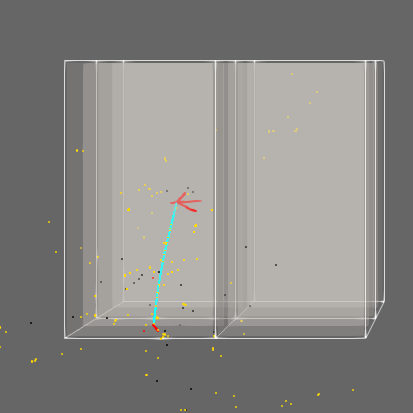
\includegraphics[width=0.45\textwidth]{{plots/EventDisplays/2.60GeV_square_crop}.png}}\hspace{25pt}
  \subfloat[$E_{\nu}$ = 3.36 GeV] {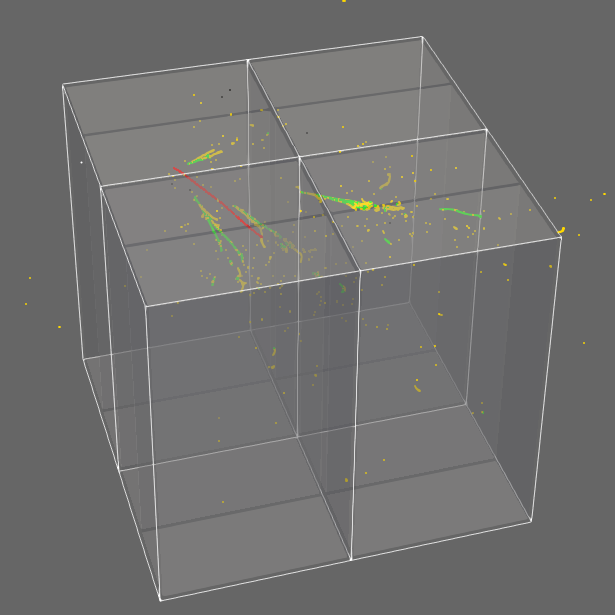
\includegraphics[width=0.45\textwidth]{{plots/EventDisplays/3.36GeV_square_crop}.png}}\\
  \subfloat[$E_{\nu}$ = 4.83 GeV] {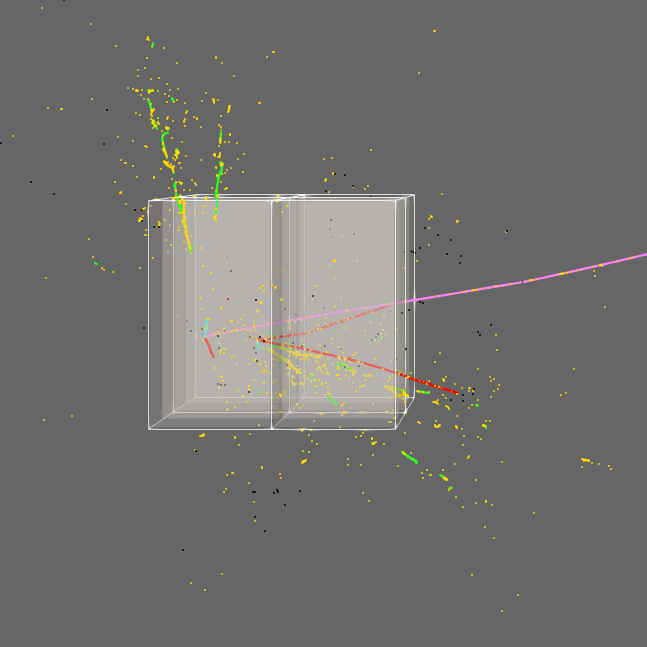
\includegraphics[width=0.45\textwidth]{{plots/EventDisplays/4.83GeV_square_crop}.png}}\hspace{25pt}
  \subfloat[$E_{\nu}$ = 9.37 GeV] {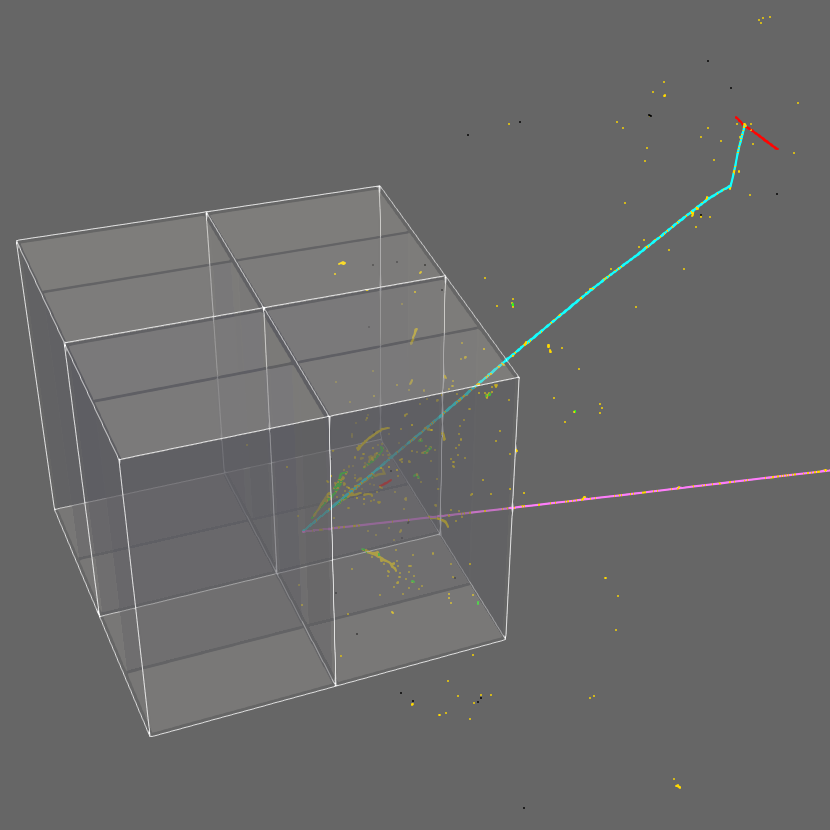
\includegraphics[width=0.45\textwidth]{{plots/EventDisplays/9.37GeV_square_crop}.png}}
  \caption{Example $\nu_{\mu}$--argon ArgonBox simulated events for a number for different incident neutrino energies, where the energy deposits in a bulk volume of LAr are color-coded according to the particle type: $\pi^{\pm}$ --- blue; $\mu^{\pm}$ --- purple; $e^{+}$ --- green; $e^{-}$ --- yellow; proton --- red; recoiling nuclei --- black. The event vertices are randomly placed within the active volume of the 2x2 Demonstrator module, the geometry for which is superimposed on these images, but which is not simulated by ArgonBox.}
  \label{fig:argonbox_event_display}
\end{figure}

The example event displays shown in Figure~\ref{fig:argonbox_event_display} give a basic idea of how NuMI ME energy events (in FHC) would look in the ArgonCube 2x2 Demonstrator module. Although many of the tracks and showers are not contained, some fraction are, which is discussed in more detail for the detector physics studies described below. It also suggests that some fraction of the events seen in the 2x2 Demonstrator module would be fully contained in the active volume, or fully contained except for the outgoing muon, which may open the way for some interesting physics studies beyond the detector physics described in this document. However, any possible utility in this direction would be severly limited without a downstream tracker to contain higher momentum hadronic components, and to tag the muon. This makes the case for adding an additional ProtoDUNE-ND test module for a HPTPC downstream tracker even stronger, or if that proves not to be possible on the timescale of this test, utilizing the existing MINERvA or MINOS-ND detectors in the experimental hall.

\begin{figure}[htb]
  \centering
  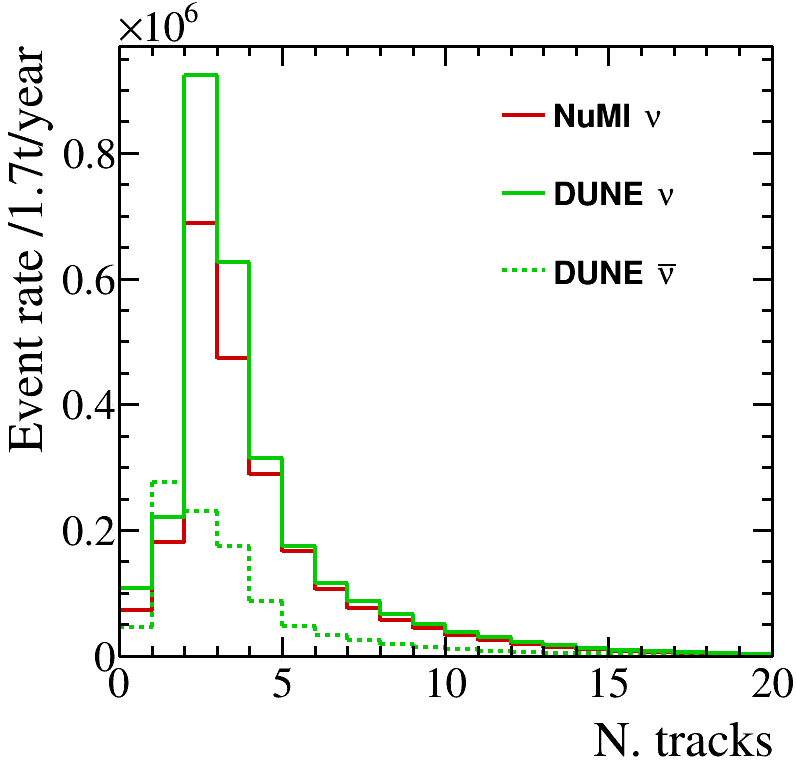
\includegraphics[width=0.5\textwidth]{plots/2x2_ntracks_all.png}
  \caption{The expected yearly rates of minimum and highly ionizing particles expected in the 2x2 Demonstrator module's 1.7t LAr volume for the NuMI ME and LBNF fluxes, produced using GENIE v2.12.10 with the ``ValenciaQEBergerSehgalCOHRES'' configuration~\cite{genie}.}
  \label{fig:track_multiplicity}
\end{figure}
In order to be a relevant test for the full ArgonCube near detector, which will be in the LBNF beamline, it is useful to verify that the basic properties of the events are similar, despite the NuMI ME beam being somewhat higher energy than the planned LBNF beam (as shown in Figure~\ref{fig:beam_options}). Figure~\ref{fig:track_multiplicity} shows the expected multiplicity of minimum or highly ionizing tracks at the vertex for both the LBNF and NuMI ME beams, in neutrino and antineutrino mode, produced with the GENIE generator. The track multiplicities are similar, which indicates that the scale of the reconstruction problem is similar, and the proposed ProtoDUNE-ND test will be a useful benchmark for developing the ArgonCube reconstruction software.

\begin{figure}[htb]
  \centering
  \subfloat[$\mu^{\pm}$] {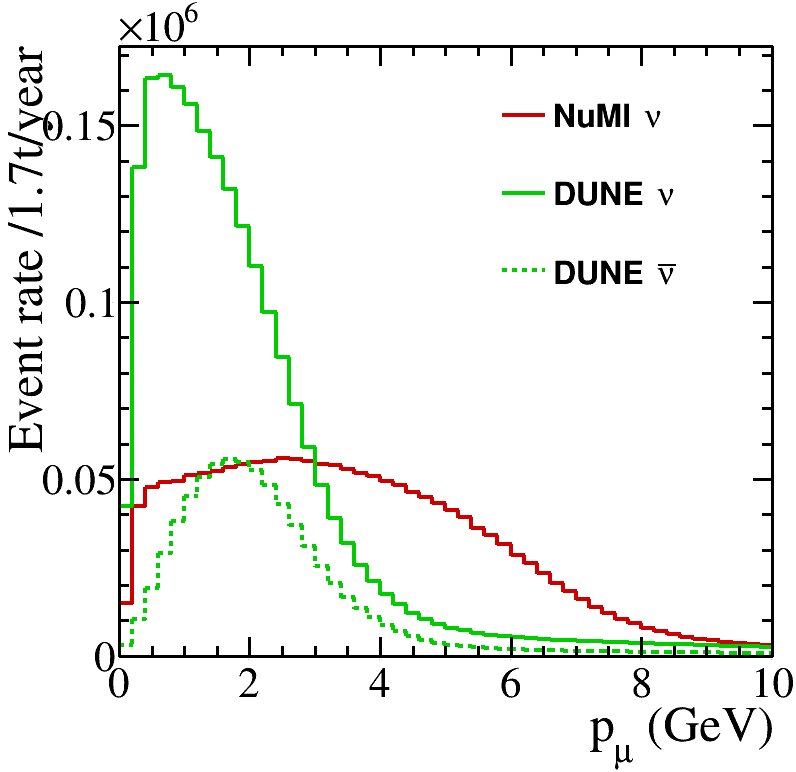
\includegraphics[width=0.5\textwidth]{plots/2x2_muon_mom_all.png}}
  \subfloat[Protons]    {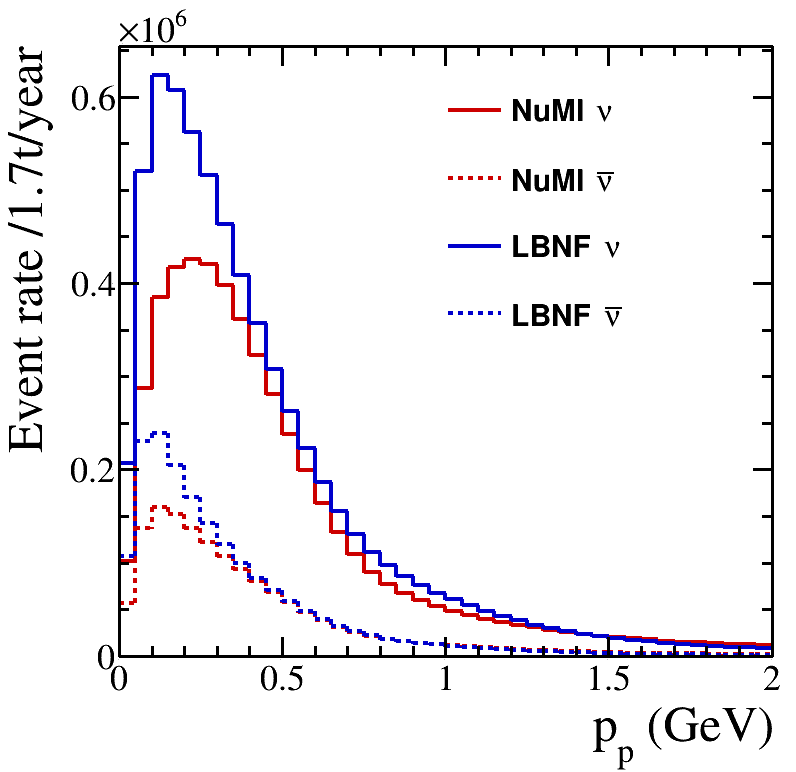
\includegraphics[width=0.5\textwidth]{plots/2x2_proton_mom_all.png}}\\
  \subfloat[$\pi^{+}$]   {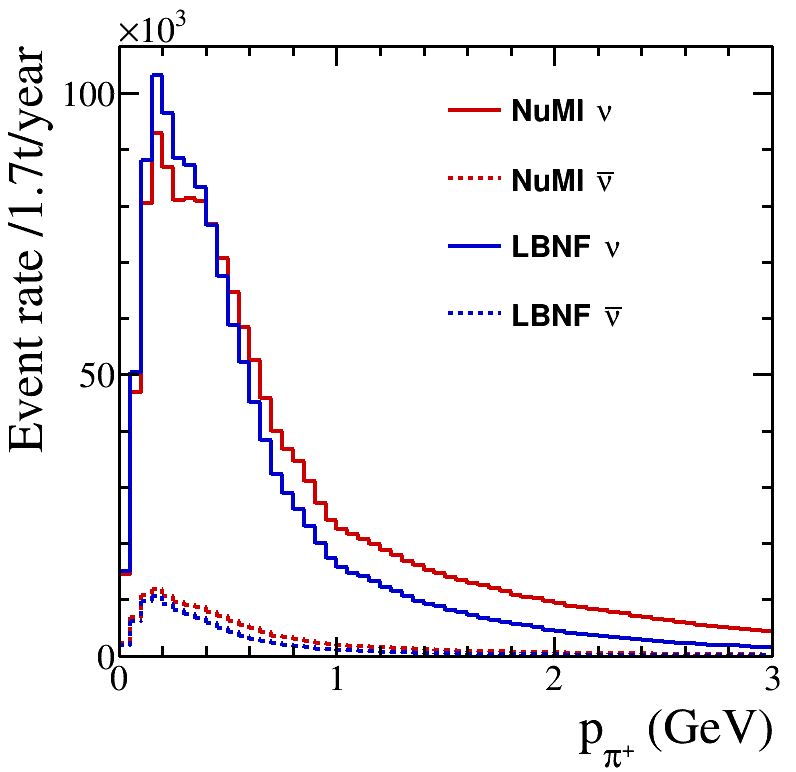
\includegraphics[width=0.5\textwidth]{plots/2x2_piplus_mom_all.png}}
  \subfloat[$\pi^{-}$]   {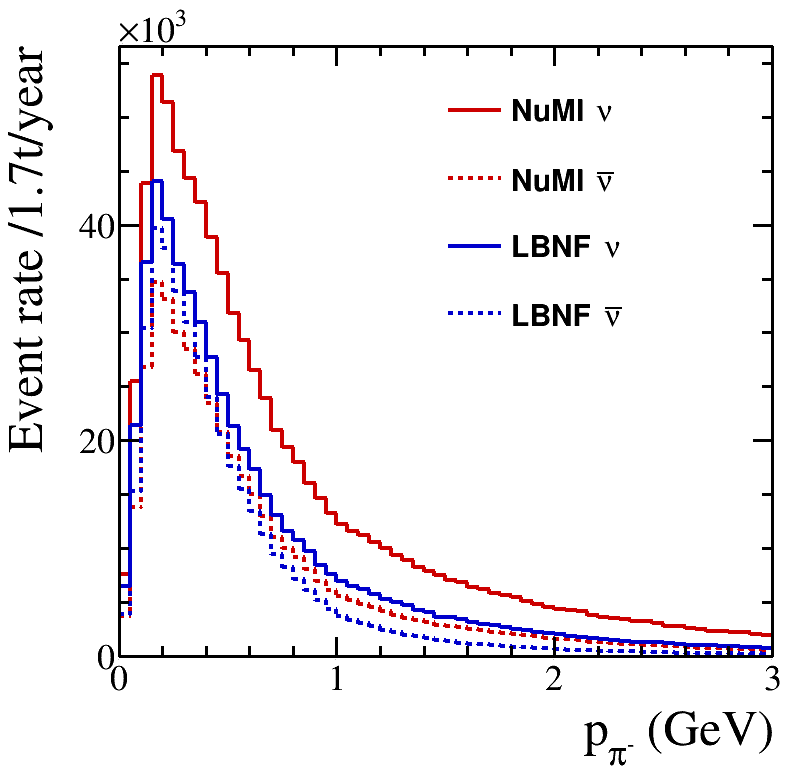
\includegraphics[width=0.5\textwidth]{plots/2x2_piminus_mom_all.png}}  
  \caption{The expected yearly rates of various particles produced at the vertex, as a function of their momentum, expected in the 2x2 Demonstrator module's 1.7t LAr volume for the NuMI ME and LBNF fluxes, produced using GENIE v2.12.10 with the ``ValenciaQEBergerSehgalCOHRES'' configuration~\cite{genie}. Note that every relevant particle from each event is included.}
  \label{fig:momenta}
\end{figure}
In Figure~\ref{fig:momenta}, the momenta of various particles coming from the initial neutrino--argon vertex are compared for the LBNF and NuMI ME beams. As expected, the energy distributions of all of the particles are slightly broader for the NuMI ME flux, but there are significant numbers of events with particle kinematics across the broad range of energies expected for the LBNF beams.

In the full 7 $\times$ 5 module ArgonCube detector and the more intense LBNF beamline, with $\sim$14.7 interactions per \SI{10}{\micro\second} beam spill makes for a very high-multiplicity environment. The entire spill will occur effectively instantaneously in the \SI{220}{\micro\second} drift window. Tracks overlapping from separate neutrino interactions is mitigated by the fully-3D readout, but association of all hits to a specific neutrino interaction can be challenging. For charged tracks, which are spatially connected to their respective neutrino interaction vertices, this association is straightforward.  However, many events contain photons and neutrons, which produce significant energy deposits that are detached from the rest of the event, and may even occur in a different ArgonCube module. Here, the ArCLight light-readout system, with the ability to measure prompt scintillation light with nanosecond resolution, will play a crucial role to associate particle tracks with the correct interaction vertices. Additionally, the relatively small size of the 2x2 Demonstrator module means that relatively few of the tracks will be contained, making particle identification (PID) studies challenging, except for the cases listed below. Although other detectors are not included in the ArgonBox simulation, the lack of containment and PID capabilities mean that including another subdetector in the ProtoDUNE-ND setup is essential for any ancillary physics measurements to be made.


\FloatBarrier
\subsection{Combining light and charge signals}
An important challenge is to develop automated event reconstruction software with the ArgonCube detector. The pixel readout removes the ambiguities present for projective wire readout TPCs, but the reconstruction software for the latter has benefitted from several years of development for the MicroBooNE~\cite{microboone} and ICARUS experiments~\cite{icarus}. Although strides forward for pixel readout TPCs have been made in the PixLAr experiment (where pixel planes were introduced to the LArIAT experiment~\cite{lariat}), the reconstruction problem for charge particle scattering in a small TPC is much simpler than for the ProtoDUNE-ND or DUNE ND environments. Additionally, the reconstructed track position along the drift direction, and the suppression of cosmic backgrounds within the beam window, will be performed using information from the ArcLight light collection system. Checking that the light and charge signals can be combined in the full-size ArgonCube modules, in a comparably noisy environment to the DUNE ND, is an essential test of the ArgonCube design.

\subsection{Neutron identification}
\label{sec:2x2_neutron}
Neutrons present a particular challenge for neutrino energy reconstruction in DUNE and other long-baseline neutrino oscillation experiments. Neutrino oscillations are a function of neutrino energy, but this cannot be reconstructed on an event by event basis because neutrons carry away some fraction of the energy, and are not directly observable. Figure~\ref{fig:neutron_kinematics} shows the expected neutron rate as a function of multiplicity and momentum for the LBNF and NuMI ME beamlines.
\begin{figure}[htb]
  \centering
  \subfloat[Neutron multiplicity]   {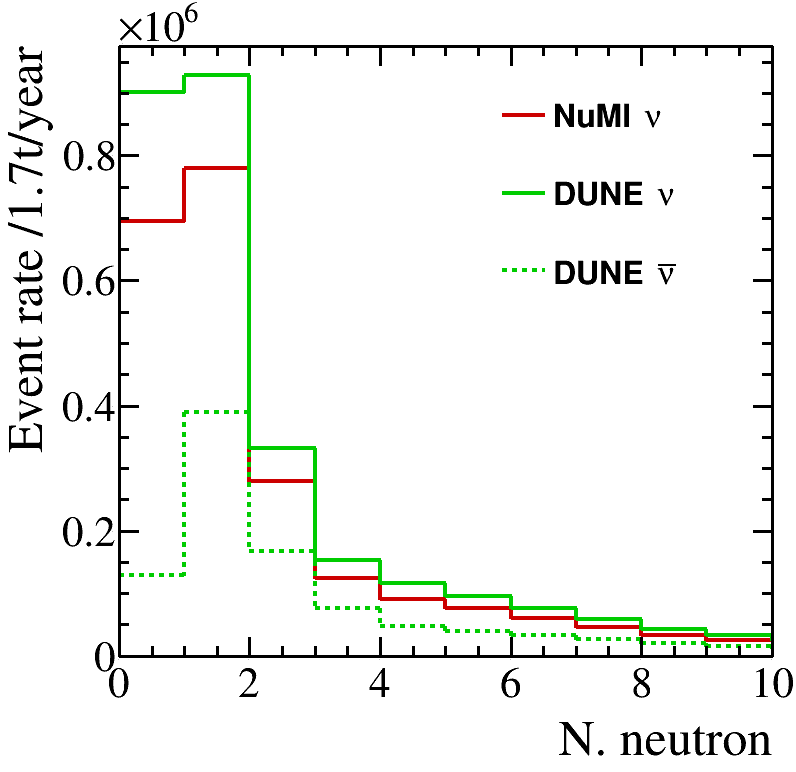
\includegraphics[width=0.5\textwidth]{plots/2x2_nneutron_all.png}}
  \subfloat[Neutron momentum]       {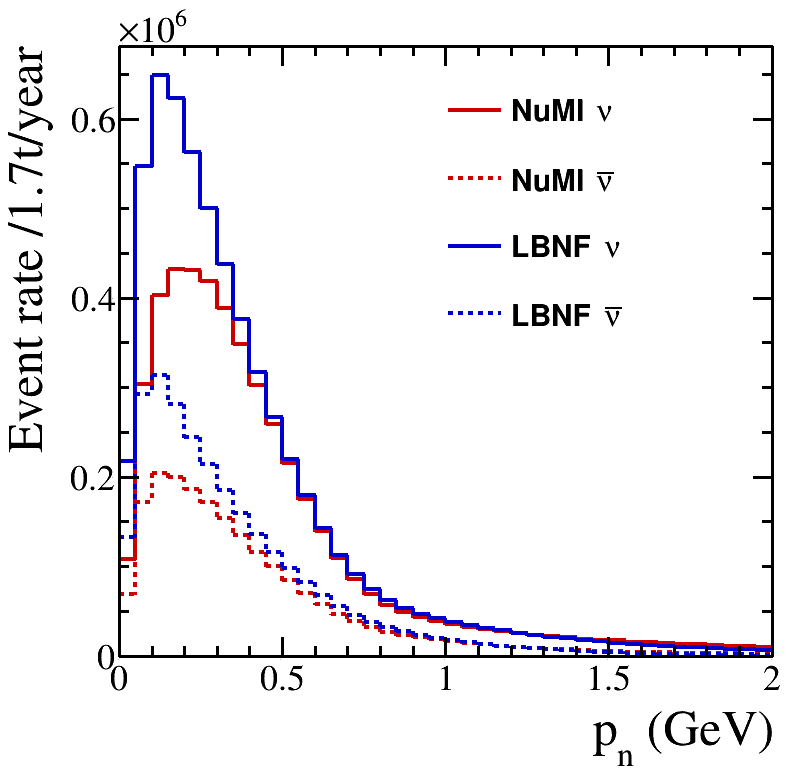
\includegraphics[width=0.5\textwidth]{plots/2x2_neutron_mom_all.png}}  
  \caption{The expected yearly rates of neutrons produced at the vertex, as a function of event multiplicity and their momentum, expected in the 2x2 Demonstrator module's 1.7t LAr volume for the NuMI ME and LBNF fluxes, produced using GENIE v2.12.10 with the ``ValenciaQEBergerSehgalCOHRES'' configuration~\cite{genie}. Note that every neutron from each event is included in the momentum distribution.}
  \label{fig:neutron_kinematics}
\end{figure}

There are two possible ways to identify the presence of neutrons in an event:
\begin{enumerate}
\item Detection of slow neutrons with kinetic energies of $\mathcal{O}$~keV through neutron capture. This is usually achieved by applying a neutron affine coating, e.g. gadolinium, to the detector walls. The radiation emitted from excited nuclei after having captured a neutron is interaction-specific and thereby serves as an indicator for slow neutrons.
\item Detection of fast neutrons with kinetic energies from $\mathcal{O}$~1 MeV-- 1 GeV through recoiling charge particles after a collision of a neutron with a nucleus. The recoiling particle can be the nucleus as a whole, or, if the neutron exceeds the nuclear binding energy ($\sim$~5~MeV for an argon nucleus), a knock-out proton or heavier nuclear fragments like deuterons.
\end{enumerate}
For oscillation experiments, fast neutrons are a much greater issue, as they may carry away a significant fraction of the neutrino energy in an event. It is, therefore, of great interest to investigate the potential of LAr experiments to tag these missing neutron with neutron-induced recoils. Investigating the neutron tagging rate in ProtoDUNE-ND will provide useful information for DUNE sensitivity studies as it will in the ProtoDUNE-ND, this provides an opportunity to investigate how well charge and light signals can be combined.

The values for pixel pitch and ArCLight threshold used in the following studies are taken from the DUNE ND proposal, although not identical to the 2x2 they are sufficiently close for the purpose of this work.  

\begin{figure}[htbp]
  \centering
  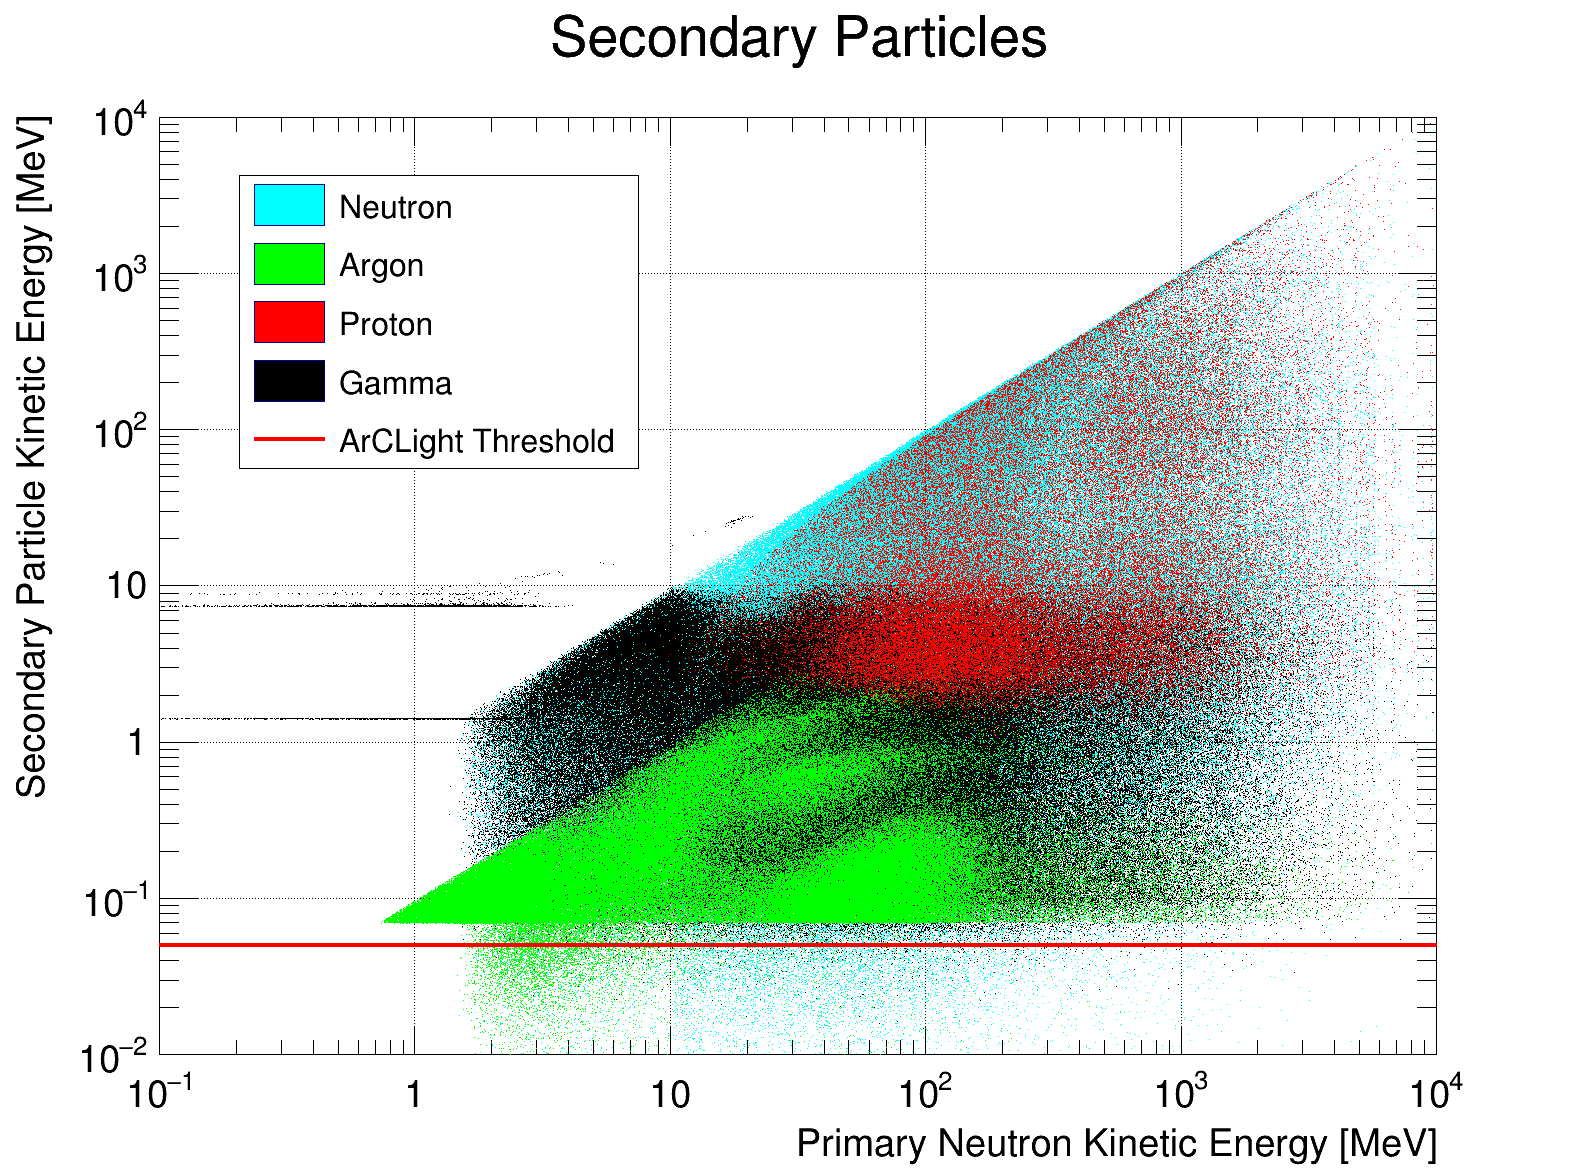
\includegraphics[width=0.8\textwidth]{plots/primary_neutron_recoils.png}
  \caption{Kinetic-energy distribution of secondary particles with respect to incident neutron kinetic energy for neutron interactions in LAr, shown for 100,000 simulated neutrino events (which may have more than one neutron produced at the vertes).}
  \label{fig:neutron_recoils}
\end{figure}
Figure~\ref{fig:neutron_recoils} shows the kinetic energy of secondary particles after the interaction of a primary neutron in LAr. The horizontal red line gives the energy threshold for the detection of these secondary particles with ArCLight~\cite{arclight}, assuming a conversion of 40k photons per MeV. Clearly, both recoiling argon nuclei and recoiling protons have kinetic energies well above the ArCLight detection threshold. While recoiling argon nuclei show typical energies between 100~keV and 1~MeV, recoiling protons show energies $>$~1~MeV, up to several GeVs.

\begin{figure}[htbp]
  \centering
  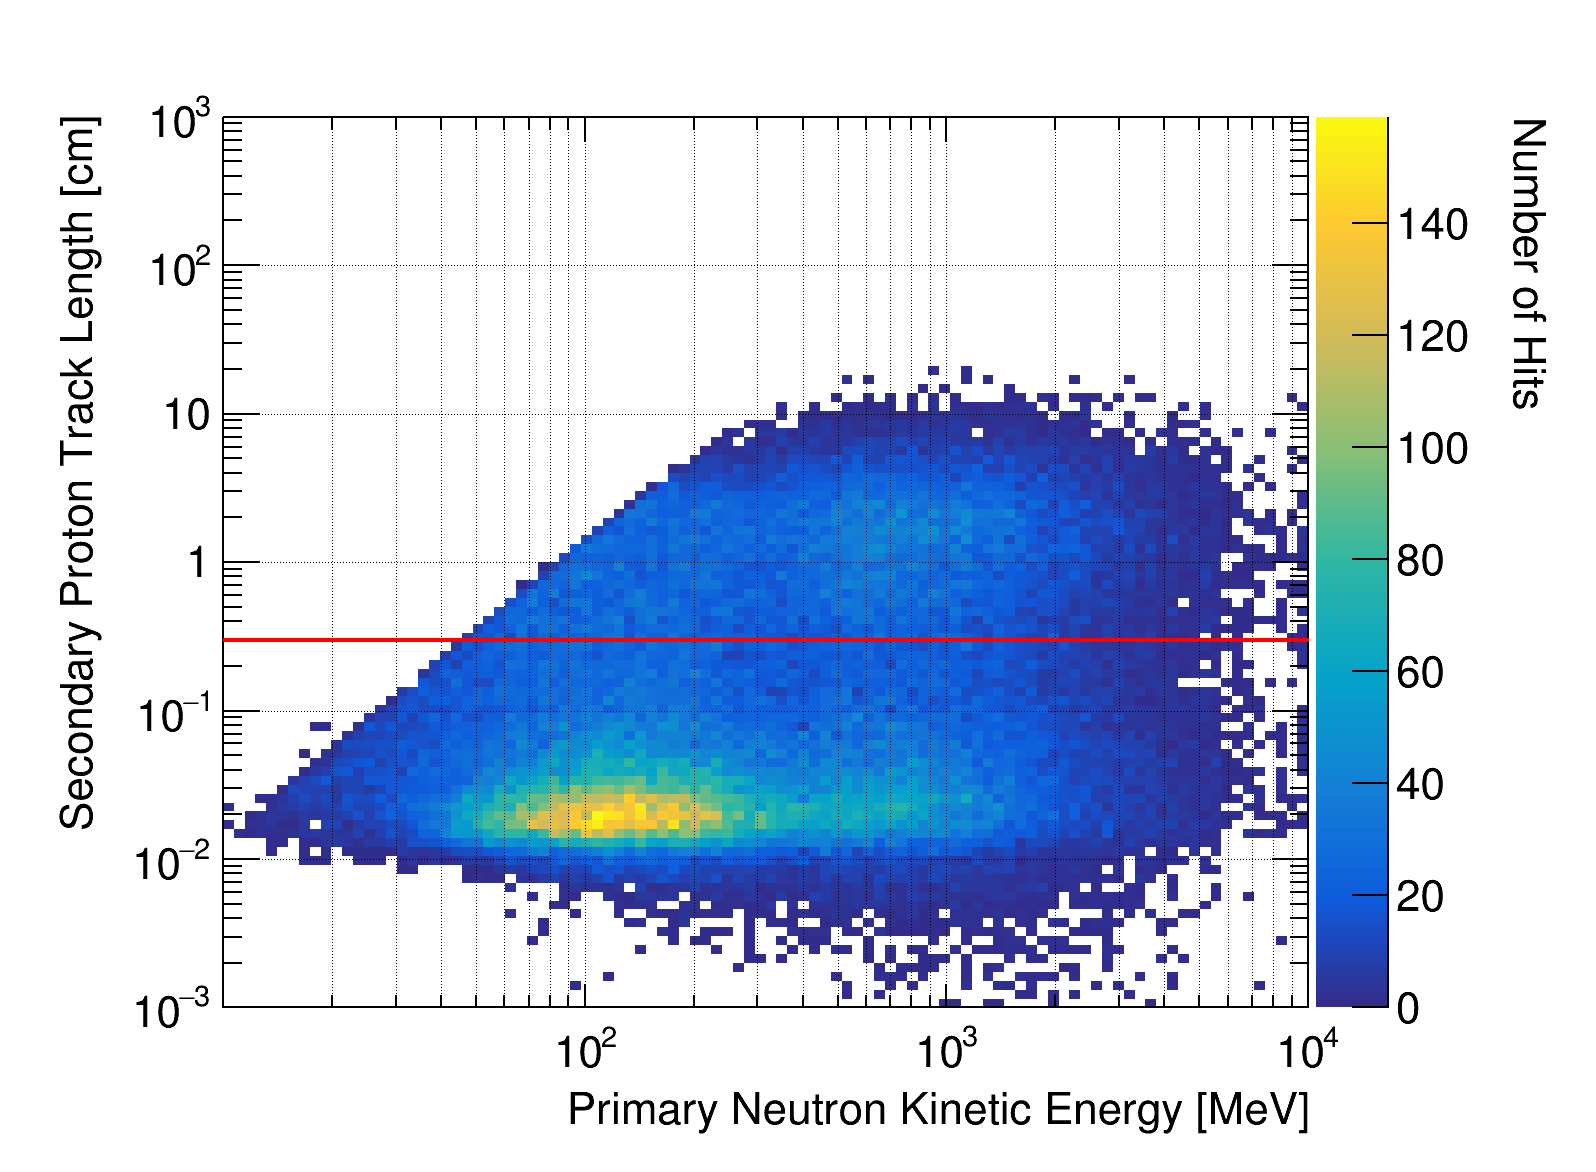
\includegraphics[width=0.8\textwidth]{plots/proton_track_length.png}
  \caption{Track length of recoiling protons for neutrons produced in 100,000 neutrino interactions. About 30\% of all recoils are resolvable as tracks with the LArPix pixel charge-readout system.The vast majority of neutron recoils contain no direction information, and will be detected only as single pixel hits.}
  \label{fig:proton_length}
\end{figure}

Given the LArPix $\sim$~3~mm pixel-pitch (see Section~\ref{sec:2x2-design}), the minimum reconstructable track length in ArgonCube is also $\gtrsim$~3~mm. Figure~\ref{fig:proton_length} shows the track length of recoiling protons with respect to the primary neutron kinetic energy. Recoiling protons can, depending on their energy, produce tracks which are up to $\sim$10~cm long. About 30~\% of all recoiling protons are resolvable by the pixelated charge readout, which correspond to protons that are knocked out of a nucleus by primary neutrons with energies $\gtrsim$~50~MeV.

\begin{figure}[htbp]
  \centering
  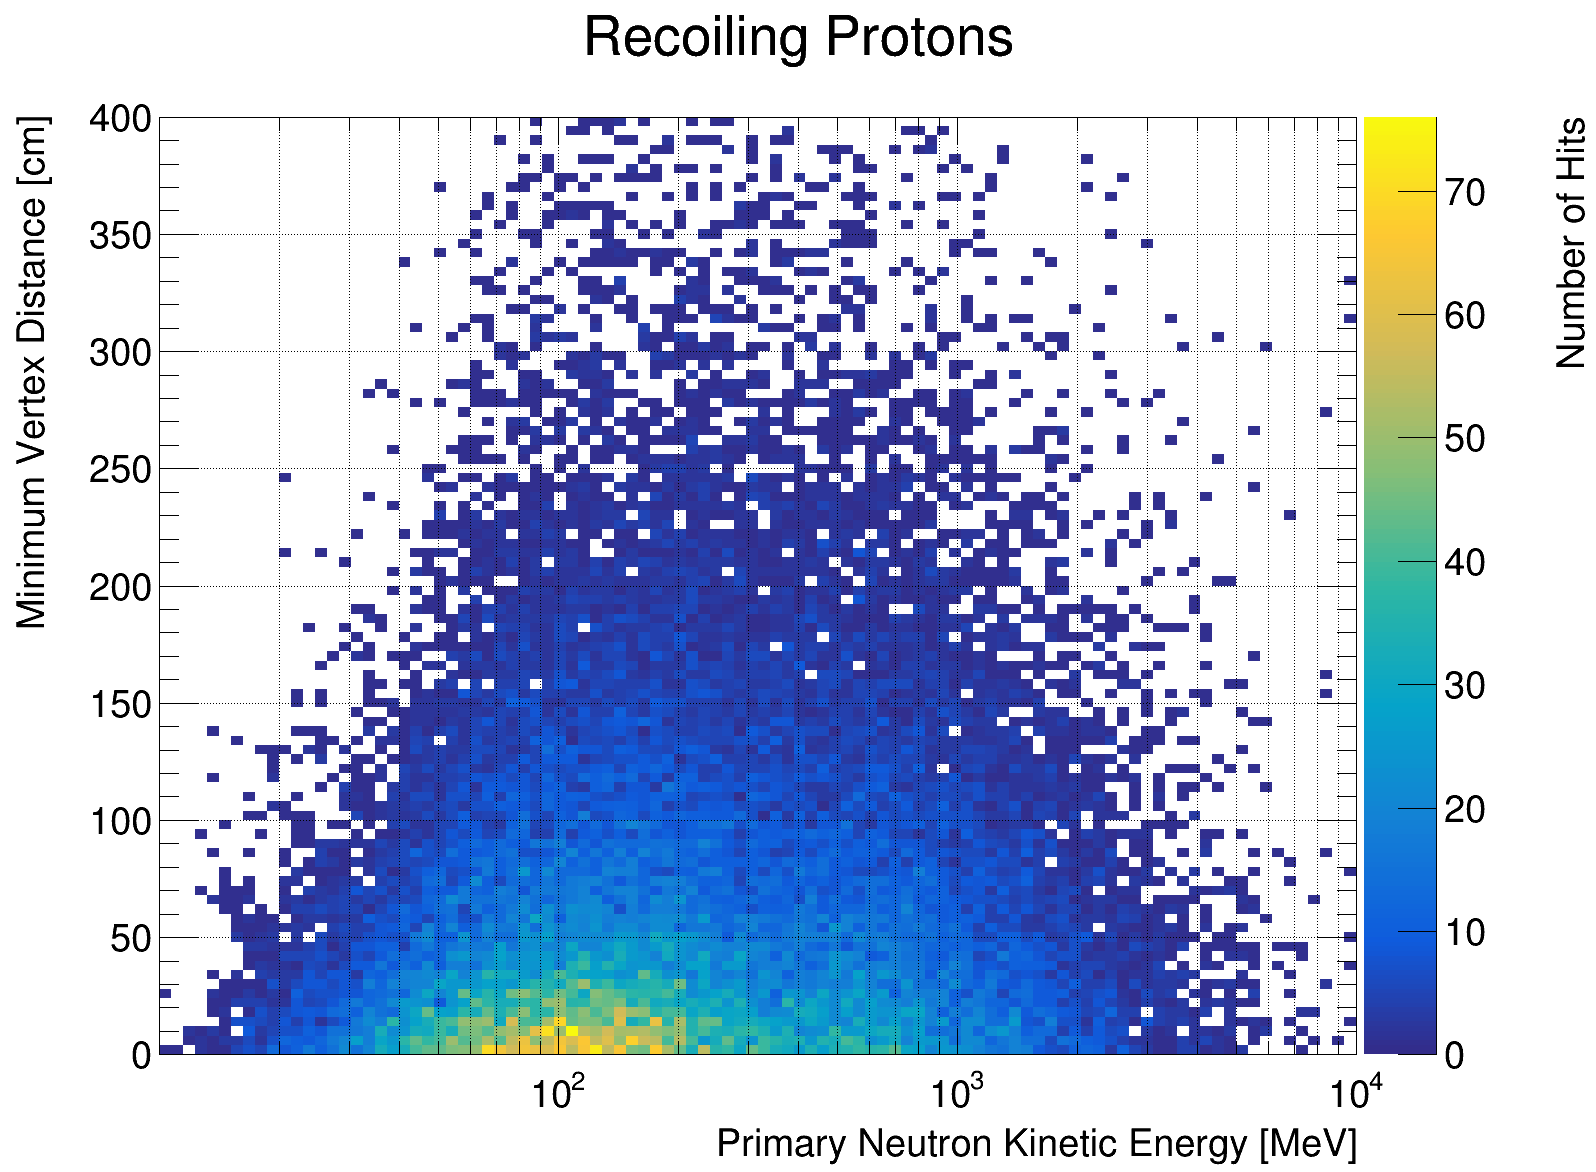
\includegraphics[width=0.8\textwidth]{plots/min_dist_vtx_proton_recoil.png}
  \caption{The minimum distance between the neutrino vertex and the neutron-induced proton track, as a function of neutron kinetic energy. Produced with 100,000 initial neutrino events simulated by ArgonBox.}
  \label{fig:min_dist_proton}
\end{figure}
Figure~\ref{fig:min_dist_proton} shows the minimum distance between the neutrino vertex and the neutron-induced proton track, as a function of neutron kinetic energy. The majority of proton recoils occur within 1 m, so many neutron-induced proton recoils will be contained within the 2x2 Demonstrator module.

\FloatBarrier
\subsection{Reconstruction in a modular environment}
The module walls of the ArgonCube design produce gaps in particle tracks traversing multiple modules. This is not the same as dead wires in classic LArTPC readouts, as it results in only $\mathcal{O}\left(10\right)\,\mathrm{mm}$ gaps in energy deposits, rather than effecting sensitivity over large areas of charge readout. Algorithms to join such segmented tracks already exist~\cite{pandora}, but have not been adapted to the ArgonCube design. Simple track matching efficiencies across modules can be calculated using cosmics, which will be an essential first step. However, for events with many tracks produced at the vertex (see Figure~\ref{fig:track_multiplicity}), a detailed study of the reconstruction performance given the module walls will need to be carried out. ProtoDUNE-ND provides an opportunity to do so, and to check that the reconstruction behaves as expected, before moving to the full DUNE ND deployment of ArgonCube.

\begin{figure}[htb]
  \centering
  \subfloat[EM shower]       {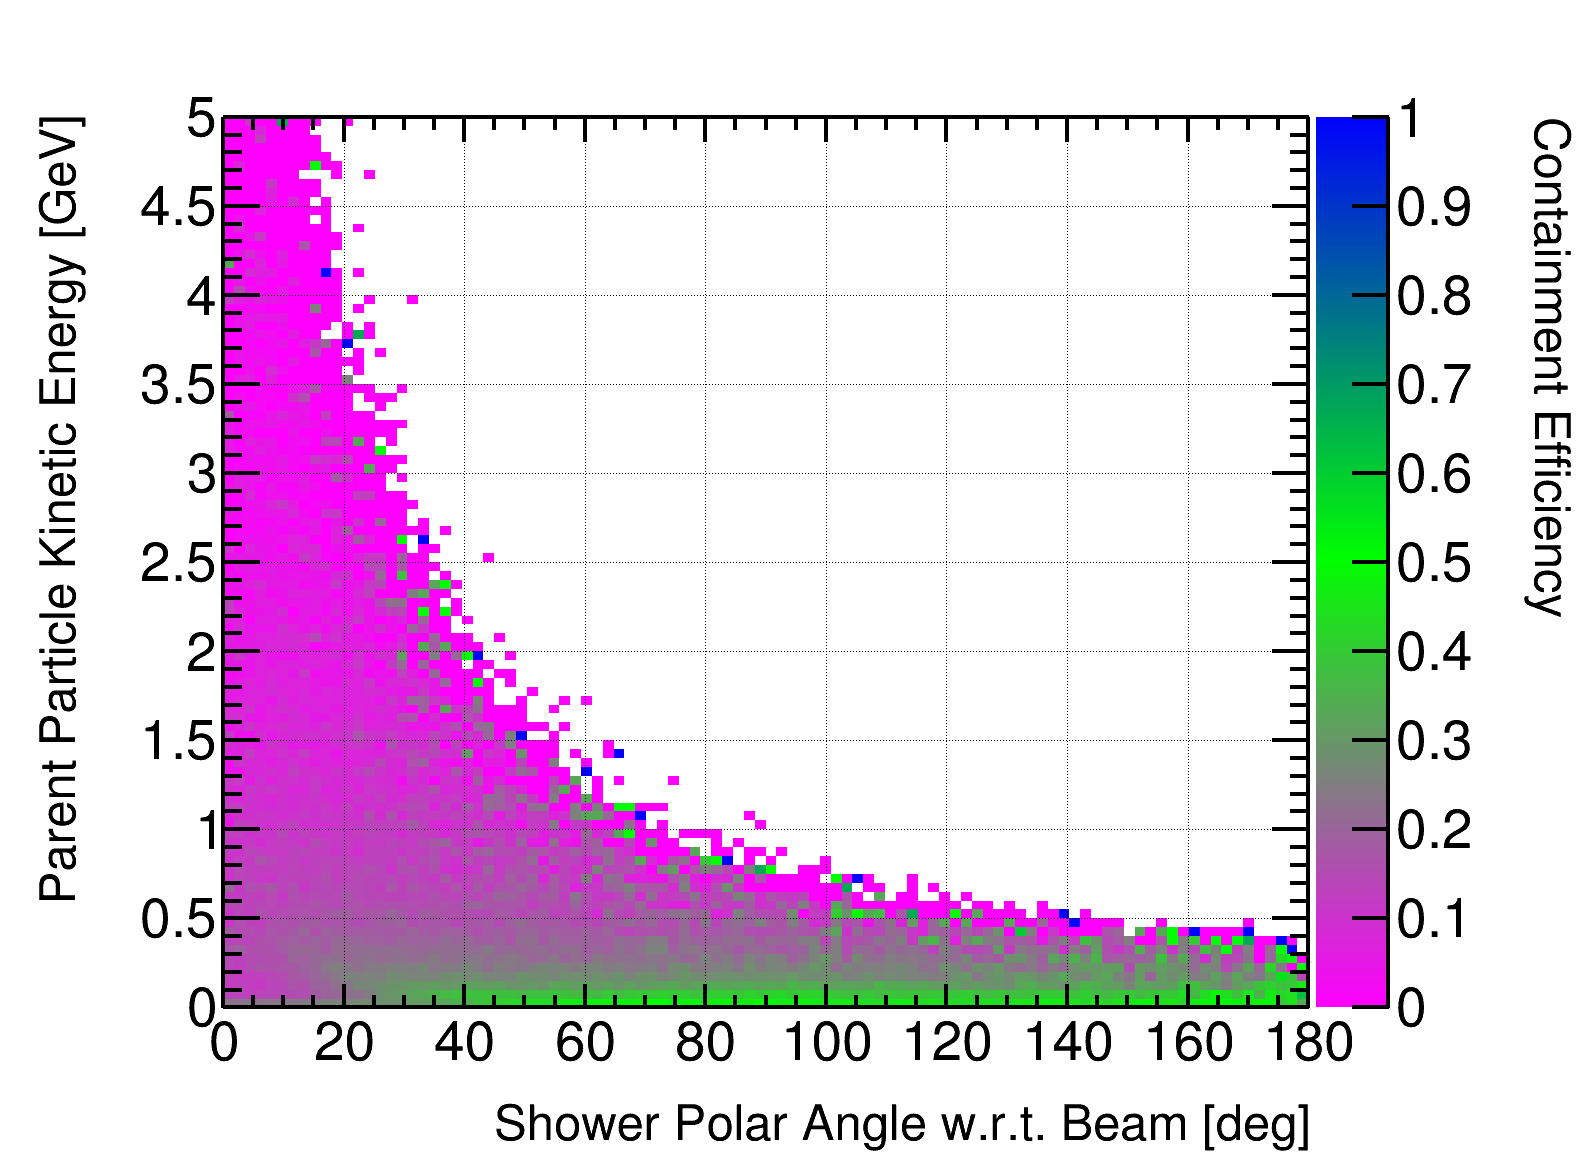
\includegraphics[width=0.5\textwidth]{plots/2x2_minerva_plots/EM_cont_eff_2x2.png}}
  \subfloat[Hadronic shower] {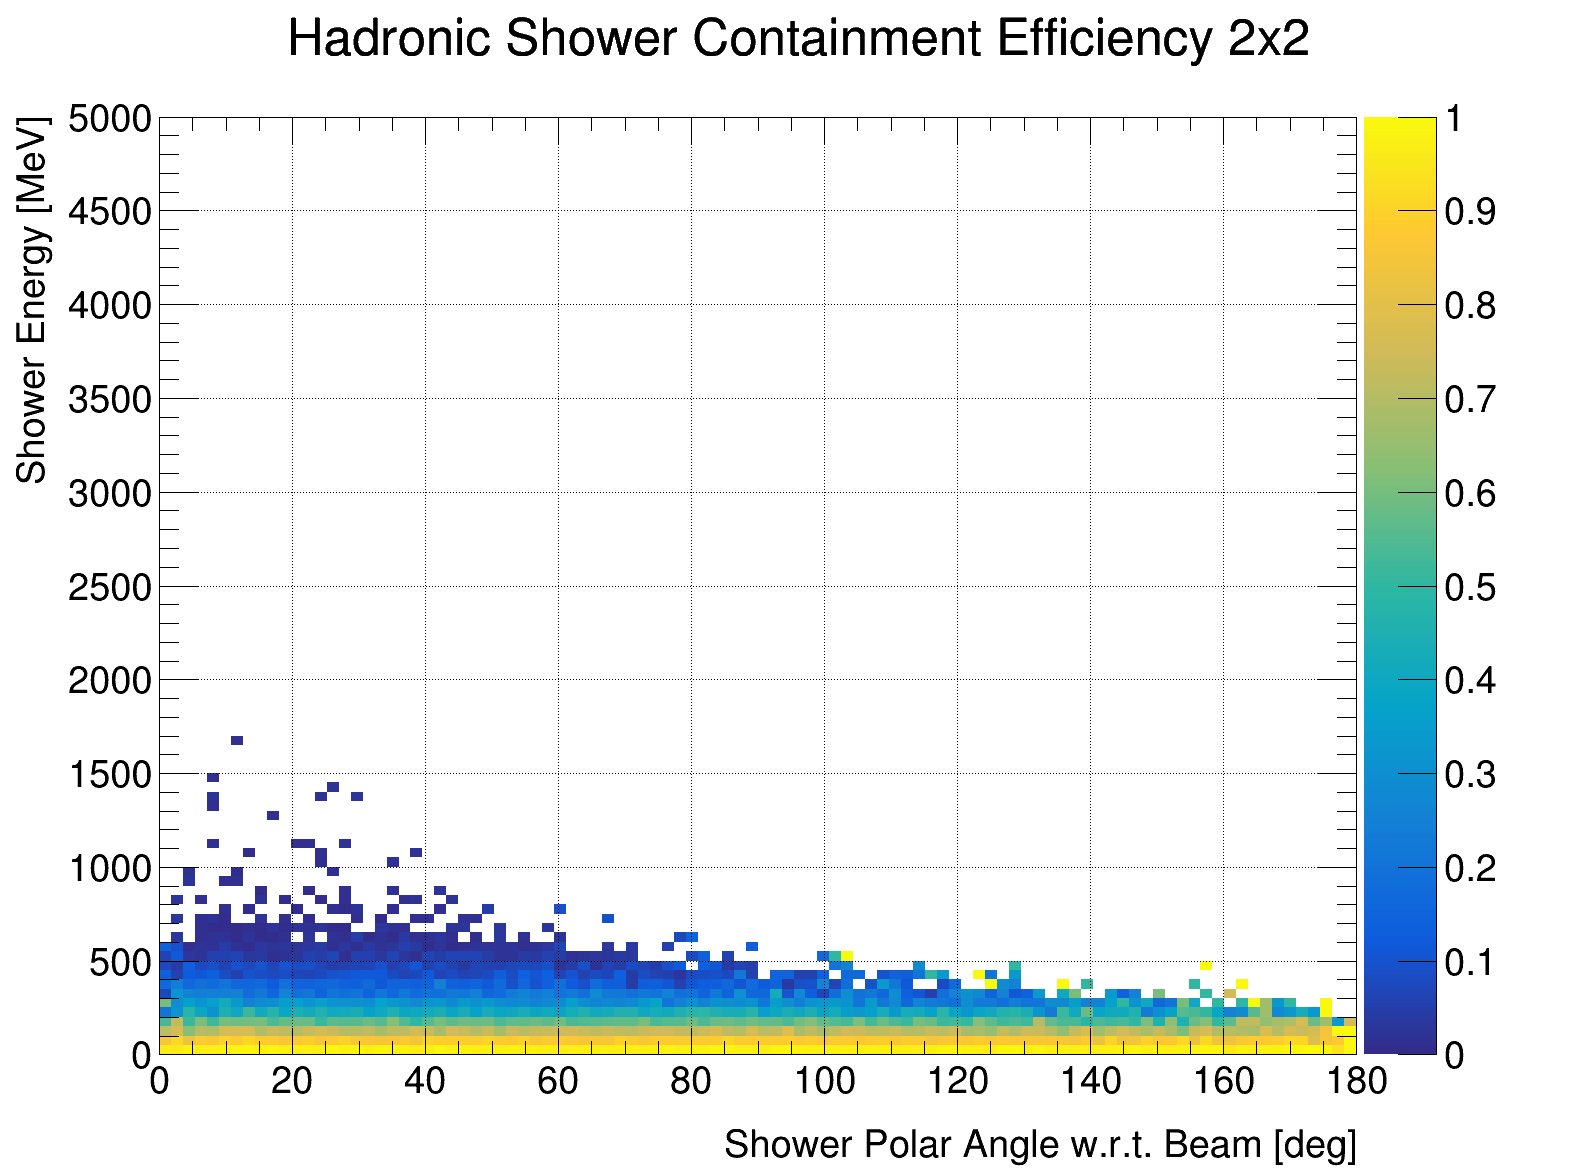
\includegraphics[width=0.5\textwidth]{plots/2x2_minerva_plots/H_cont_eff_2x2.png}}
  \caption{Containment efficiency for EM and hadronic showers produced by an interaction within the ArgonCube 2x2 active volume, as a function of initiator particle energy and angle w.r.t the incoming beam direction. Note that if $\geq 90$\% of energy is deposited within the 2x2 active volume, it is classed as contained.}
  \label{fig:2x2_shower_containment}
\end{figure}
This problem becomes significantly more complicated for electro-magnetic (EM), or hadronic, showers which cross modules. ProtoDUNE-ND will provide an opportunity to develop reconstruction software, and check how well it performs for realistic shower energies for neutrino interactions which cover the neutrino energy range of interest for the LBNF beamline. At these energies, shower development is known to be problematic, and shower reconstruction in LAr is a significant challenge. Additionally, in order to test how well the reconstruction can identify shower depth, a sample of fully contained showers would be extremely useful. Figure~\ref{fig:2x2_shower_containment} shows the efficiency to fully contain EM-showers or hadronic showers produced by an interaction within the ArgonCube 2x2 active volume, as a function of initiator particle energy and angle w.r.t the incoming beam direction. Note that if $\geq 90$\% of energy is deposited within the 2x2 active volume, it is classed as contained. 

\todo{Add some event displays.}

\todo{Patrick, James, can you think of anything else here? Seems a bit weak on the shower study...}

\subsection{$\pi^{0}$ reconstruction}
A more quantitative measure of how well EM showers can be reconstructed in the modularized ArgonCube detector could be possible using $\pi^{0} \rightarrow \gamma\gamma$ decays (which have a branching ratio of 98.8\%~\cite{pdg_2018}), in which both decay photons produce a shower, and are contained in the active volume of the detector. Combining the information on the two showers, and attempting to reconstruct the invariant mass peak of the $\pi^{0}$ provides a measurement of the EM shower resolution.

\begin{figure}[htb]
  \centering
  \subfloat[$\pi^{0}$ multiplicity]   {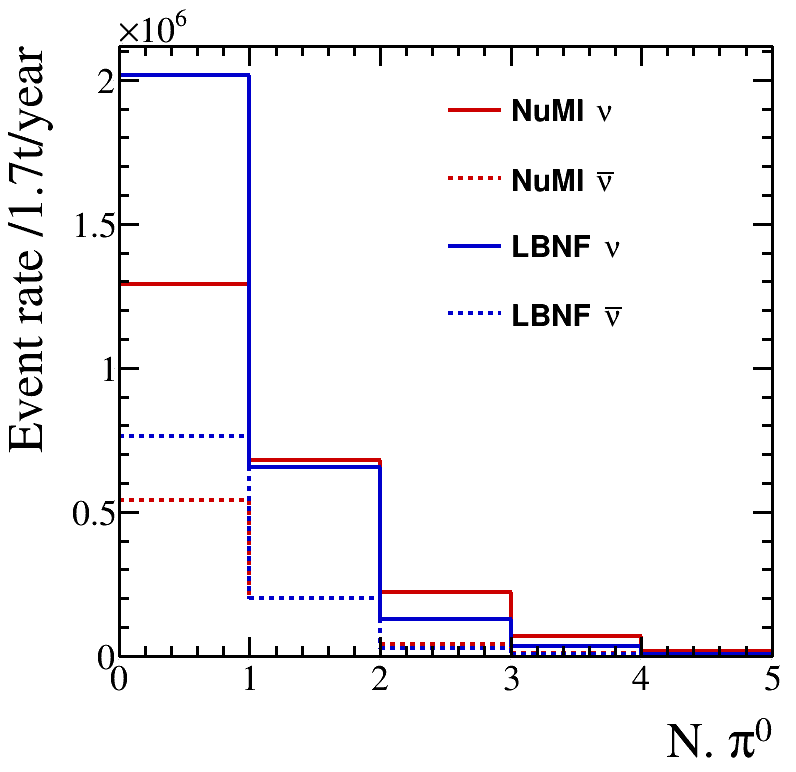
\includegraphics[width=0.5\textwidth]{plots/2x2_npi0_all.png}}
  \subfloat[$\pi^{0}$ momentum] {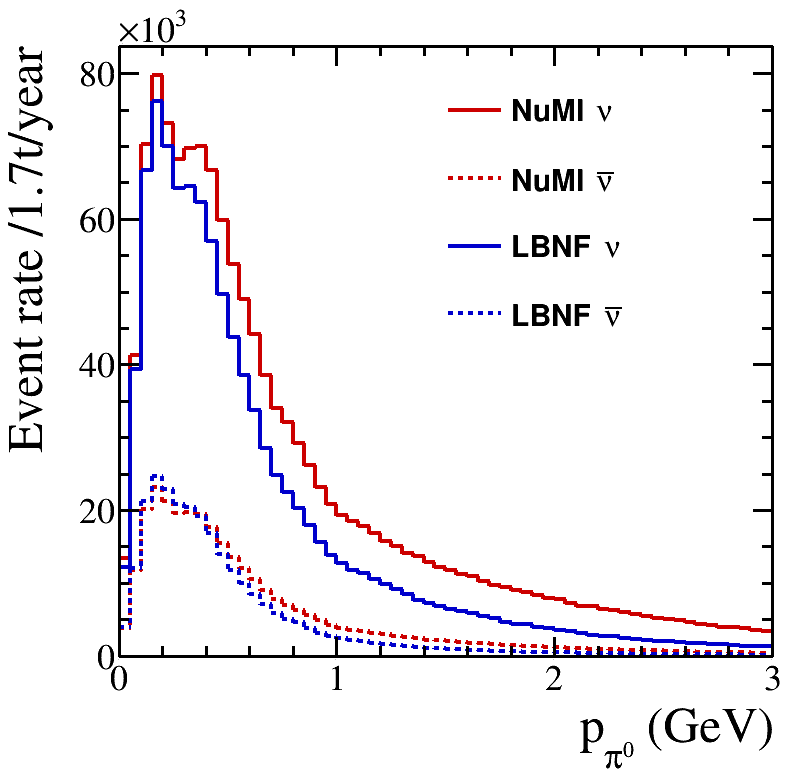
\includegraphics[width=0.5\textwidth]{plots/2x2_pi0_mom_all.png}}  
  \caption{The expected yearly rates of $\pi^{0}$'s produced at the vertex, as a function of event multiplicity and their momentum, expected in the 2x2 Demonstrator module's 1.7t LAr volume for the NuMI ME and LBNF fluxes, produced using GENIE v2.12.10 with the ``ValenciaQEBergerSehgalCOHRES'' configuration~\cite{genie}. Note that every $\pi^{0}$ from each event is included in the momentum distribution.}
  \label{fig:pi0_kinematics}
\end{figure}
Figure~\ref{fig:pi0_kinematics} shows the expected $\pi^{0}$ production rate in the active volume of the 2x2 Demonstrator module in the LBNF NuMI ME beamlines, as a function of $\pi^{0}$ multiplicity in each event and $\pi^{0}$ momentum. There are, of course, some qualifiers for this study. Many photon-induced showers will not be contained, and those which are will be lower energy than many EM showers expected in the DUNE ND. Figure~\ref{fig:pi0_containment_2x2} shows the efficiency for containing both photon-induced showers from a primary $\pi^{0}$ decay in the ArgonCube 2x2's active volume, shown for all $\pi^{0}$'s produced inside that volume. As expected, the efficiency is low for high energy pions, but it will still be possible to reconstruct a large fraction of the lower momentum $\pi^{0}$'s from Figure~\ref{fig:pi0_kinematics}. Overall, this study shows that this $\pi^{0}$ mass peak reconstruction will be a worthwhile study at ProtoDUNE-ND.

\begin{figure}[htb]
  \centering
  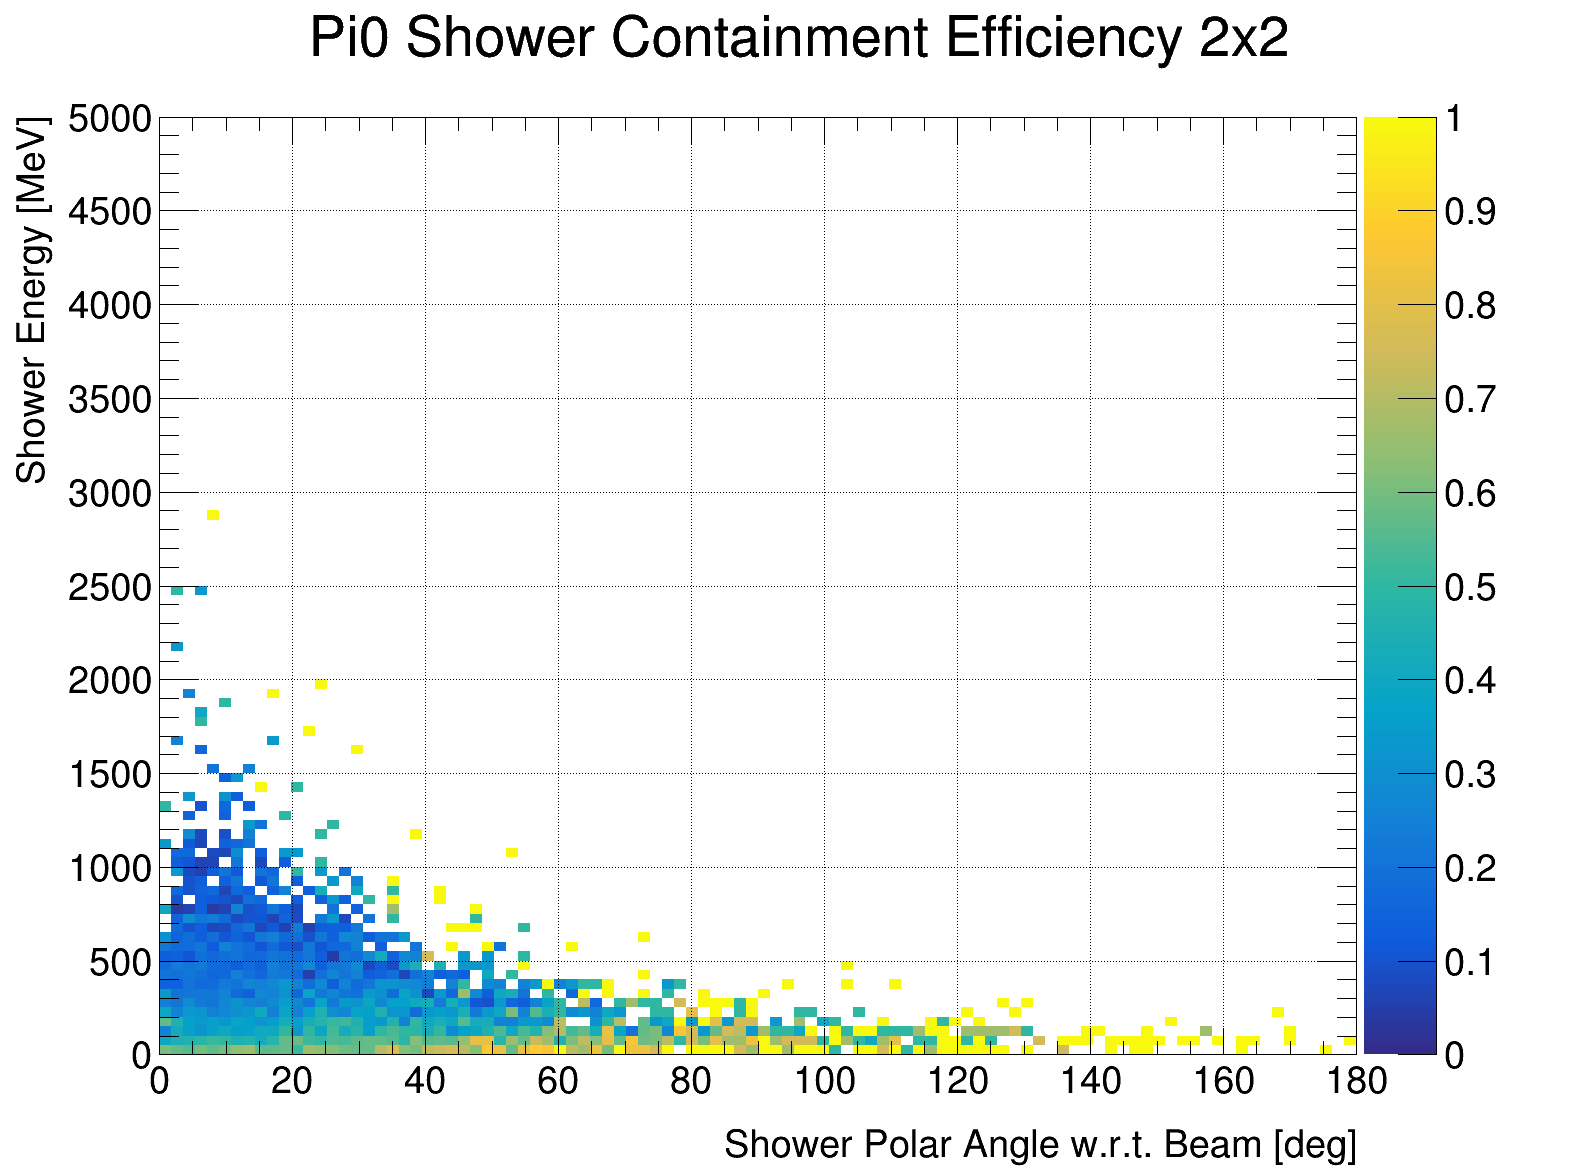
\includegraphics[width=0.5\textwidth]{plots/2x2_minerva_plots/Pi0_cont_eff_2x2.png}
  \caption{Efficiency for containing both photon-induced showers from $\pi^{0}$ decays in the ArgonCube 2x2 module, as a function of the $\pi^{0}$ kinetic energy and angle w.r.t the incoming neutrino direction. Containment is defined as $\geq$90\% of the energy being deposited in an active volume of a detector, and all primary $\pi^{0}$'s produced inside the 2x2's active volume are included.}
  \label{fig:pi0_containment_2x2}
\end{figure}
Two further issues for this study are apparent. Firstly, events with more than one $\pi^{0}$ introduce a problem: even if two EM showers are fully contained, they may not come from the same $\pi^{0}$ decay. Secondly, of those $\pi^{0}$ decays for which both photons are fully contained, the initial $\pi^{0}$ is likely to have a low momentum, which is likely to exclude some fraction of the events. However, despite these challenges, a measure of EM shower resolution from ProtoDUNE-ND would be very useful for DUNE ND design studies, so this possibility is worth investigating further.

Studies have shown that a 3D-charge readout will improve reconstruction of $\pi^{0}$ showers by removing energy deposits from events crossing the shower~\cite{Damian}. However, as for any LArTPC a first step for the 2x2 will be to demonstrate electron-photon separation near the vertex.    

\label{sec:efield}
A concern for LAr detectors in a high intensity beam is the build up of space charge --- long-lived argon ions which drift slowly towards the cathode --- and possible affects on the uniformity of the electric field which may accumulate over time. In currently operating and near-future LAr detectors~\cite{Ereditato:2014lra, Antonello:2015lea}, both cosmic tracks and UV lasers are used to calibrate for distortions in the electric field. Both the UV laser track and high energy cosmic muons are expected to leave straight tracks in the detector. If the drift field is not uniform across the detector, ionization electrons produced along the length of this track will not drift at the same speed, and will result in a distorted track at the readout plane. By comparing the reconstructed and expected track, a map of the electric field distortion can be built up for calibration purposes.

Assuming that the 2x2 Demonstrator module is equipped with scintillator panels to tag cosmic tracks using a timing coincidence between two sides of the detector, and reasonable spatial resolution on those scintillator paddles, electric field distortions could be measured in the 2x2 Demonstrator module. By looking at beam-on, and beam-off data, it would be possible to look at the possible affect of space charge build-up over time due to the high event rate in the NuMI beam. If significant space charge build-up were observed, this would inform the future ArgonCube ND design, as a higher drift field strength would be required.

Additionally, although the electric-field uniformity of the resistive field shell will be checked in a small scale LAr TPC at Bern, a check of the electric-field uniformity and stability over time for full-size ArgonCube modules would be a valuable final validation of the design.

\subsection{Cosmic and Rock Muon suppression}
\label{sec:cosmic-suppression}

The DUNE ND is located underground with a \SI{50}{\metre} overburden, that reduces the cosmic flux by orders of magnitude compared to surface detectors. The cosmic rate in MINERvA is \SI{18}{\hertz}, for $\sim$\SI{6}{\metre\squared}.  For 2x2, the $\sim$\SI{150}{\micro\second} readout window, assuming $\sim$\SI{2}{\metre\squared}, the rate of cosmics muons is 0.001 per readout window. Reading out around spills only, will result in a coincident cosmic muon once every 20 minutes.
In DUNE ND we expect $\sim$10 rock muons per spill, which will be on average $\sim$\SI{1}{\micro\second} apart in time. They will not overlap any neutrino activity in 3D, but the fast timing will provide an additional handle.
A key design choice for the DUNE ND is whether or not a muon tagging system is required --- for example, a series of scintillator planes surrounding the LAr TPC, as for SBND and MicroBooNE~\cite{CRT}. The proposed ProtoDUNE-ND test experiment can help inform this design choice, assuming that the ArgonCube 2x2 Demonstrator module is equipped with scintillator paddles.

By using the scintillator paddles to tag cosmic or rock events using a timing coincidence, methods for rejecting them can be validated independently. For example, we expect that the good timing resolution and light localization from ArcLight will allow cosmics out of the beam window to be rejected with a high efficiency. Additionally, if a cosmic muon traverses a pixel plane, or an ArcLight plane, we would expect to see a large charge deposition or a large number of photoelectrons measured, which could be an additional way to reject cosmic muons. Both of these methods can be validated with ProtoDUNE-ND.

\subsection{Reconstruction with multiple subdetectors}
Because the ArgonCube 2x2 Demonstrator module is relatively small, many events from the NuMI ME beam will not be contained. Figure~\ref{fig:leaky_event} shows a neutral current event where many pions are produced, but in which the pions and subsequent hadronic showers extend far beyond the detector. Such events are likely to be uncontained even in the full ArgonCube component of the DUNE ND. In charged-current events, the muon will be uncontained most of the time. For this reason, and because it is not possible to magnetize the large LAr component, a magnetized tracking detector is proposed downstream of ArgonCube in the DUNE ND. A test module for the HPTPC is hoped to be included as part of the ProtoDUNE-ND effort as described in Section~\ref{sec:tracking_detectors}. With multiple subdetectors included in ProtoDUNE-ND, multi-detector reconstruction capabilities can be developed and tested. Additionally, if the sign and momentum of escaping hadrons and muons can be measured, it may be possible to make physics measurements with ProtoDUNE-ND, which would be beneficial to the overall DUNE program. For that reason, if no downstream tracker is available, it would be highly desirable to utilize the proximity of the MINERvA and MINOS-ND detectors, and try to minimize the distance between the ArgonCube 2x2 Demonstrator module and those detectors, in order to use them as downstream trackers.
\begin{figure}[htb]
  \centering
  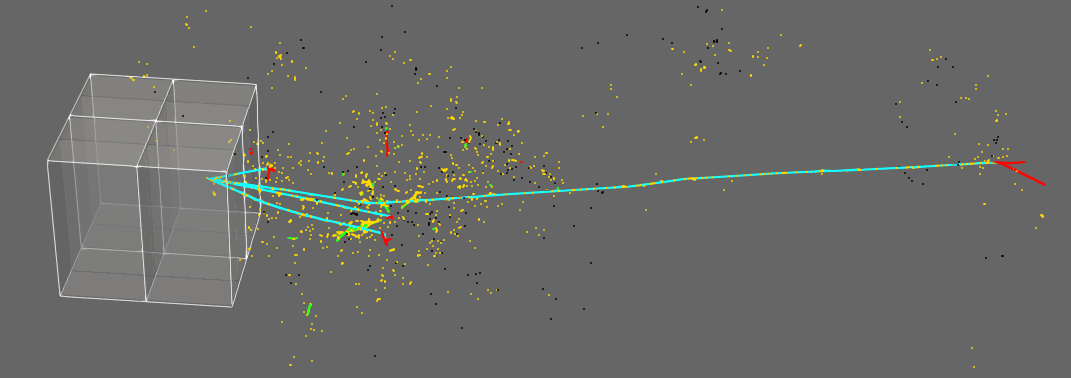
\includegraphics[width=0.8\textwidth]{{plots/EventDisplays/8.17GeV_rectangle_crop}.png}
  \caption{Example ArgonBox simulated event for an 8.17 GeV $\nu_{\mu}$--argon neutral-current multi-pion interaction, in which the pions are not contained in the module. Energy deposits in a bulk volume of LAr are color-coded according to the particle type: $\pi^{\pm}$ --- blue; $\mu^{\pm}$ --- purple; $e^{+}$ --- green; $e^{-}$ --- yellow; proton --- red; recoiling nuclei --- black. The event vertex was randomly placed inside the active volume of the 2x2 Demonstrator module, the geometry for which is superimposed on these images, but which is not simulated by ArgonBox.}
  \label{fig:leaky_event}
\end{figure}
\FloatBarrier
